% Created 2022-06-23 Thu 17:12
% Intended LaTeX compiler: pdflatex
\documentclass[11pt]{article}
\usepackage[utf8]{inputenc}
\usepackage[T1]{fontenc}
\usepackage{graphicx}
\usepackage{longtable}
\usepackage{wrapfig}
\usepackage{rotating}
\usepackage[normalem]{ulem}
\usepackage{amsmath}
\usepackage{amssymb}
\usepackage{capt-of}
\usepackage{hyperref}
\author{Ali, Mihir, Noah}
\date{\today}
\title{Einführung in die Theoretische Informatik Zusammenfassung}
\hypersetup{
 pdfauthor={Ali, Mihir, Noah},
 pdftitle={Einführung in die Theoretische Informatik Zusammenfassung},
 pdfkeywords={},
 pdfsubject={},
 pdfcreator={Emacs 28.1 (Org mode 9.6)}, 
 pdflang={English}}
\begin{document}

\maketitle
\tableofcontents


\section{Formale Sprachen}
\label{sec:org027349c}

\subsection{Grundbegriffe}
\label{sec:org0d79b1f}
\begin{itemize}
\item Alphabet \(\Sigma\) (endliche Menge) z.B. \(\{1,0\}\)
\item Wort/String über \(\Sigma\) ist eine endliche Folge von Zeichen aus \(\Sigma\)
\item \(|w|\) länge des Wortes \(w\)
\item Leeres Wort \(\epsilon\)
\item \(uv\) konkatenation der Wörter \(u\) und \(w\)
\item Ist \(w\) ein Wort so ist \(w^0 = \epsilon\) und \(w^{n+1} = ww^n\)
\item \(\Sigma^*\) Menge aller Wörter über \(\Sigma\)
\item (formale) Sprache \(L \subseteq \Sigma^*\)
\end{itemize}

\subsubsection{Operationen auf Sprachen}
\label{sec:org8bcdd5b}
Seien \(A,B \subseteq \Sigma^*\)
\begin{itemize}
\item Konkatenation:
\end{itemize}
\(AB = \{uv | u \in A \land v \in B \}\)
\begin{itemize}
\item Konkatenation mit sich selbst:
\end{itemize}
\(A^n = \{w_1 ... w_n | w_1, ... , w_n \in A\} = A ... A\)
\begin{itemize}
\item \(A^* = \{w_1...w_n | n \geq 0 \land w_1, ... , w_n \in A\} = \bigcup_{n\in \mathbb{N}} A^n\)
\item \(A^+ = AA^* = \bigcup_{n \geq 1} A^n\)
\end{itemize}
\begin{enumerate}
\item Sonderfälle:
\label{sec:org93c2fa2}
\begin{itemize}
\item \(\forall A: \epsilon \in A^*\)
\item \(\emptyset^* = \{\epsilon\}\)
\item \(\emptyset A = \emptyset\)
\item \(\{\epsilon \} A = A\)
\item \(A^*A^* = A^* = (A^*)^*\)
\end{itemize}
\end{enumerate}

\subsubsection{Grammatiken}
\label{sec:org1e41910}
4-Tupel \(G = (V,\Sigma,P,S)\)
\begin{itemize}
\item \(V\) ist endliche Menge von Nichtterminalzeichen
\item \(\Sigma\) ist endliche Menga von Terminalzeichen (= Alphabet)
\item \(P \subseteq (V \cup \Sigma)^* \times (V \cup \Sigma)^*\) ist Menge von Produktionen
\item \(S \in V\) ist das Startsymbol
\end{itemize}

Die Sprache von G ist die Menge aller Wörter, die von G erzeugt werden. Sie wird mit \(L(G)\) bezeichnet.
Also jedes Wort, dass die Grammatik erzeugt muss in der Sprache erhalten sein und jedes Wort in der Sprache muss von der Grammatik erzeugt werden.
\begin{enumerate}
\item Reflexve transitive Hülle
\label{sec:org4b7d4fd}

\begin{itemize}
\item \(\alpha \rightarrow^0_G \alpha\)
\item \(\alpha \rightarrow^{n+1}_G \gamma: \exists \beta. \alpha \rightarrow^n_G \rightarrow_G \gamma\)
\item \(\alpha \rightarrow^{*}_G \beta : \exists n. \alpha \rightarrow^n_G \beta\)
\item \(\alpha \rightarrow^{+}_G \beta: \exists n>0. \alpha \rightarrow^n_G \beta\)
\end{itemize}
\end{enumerate}

\subsubsection{Chomsky Hierarchie}
\label{sec:org7350668}
Eine Grammatik G ist vom
\begin{itemize}
\item Typ 0 immer
\item Typ 1 falls fpr jede Produktion \(\alpha \rightarrow \beta\) außer \(S \rightarrow \epsilon\) gilt \(|\alpha| \leq |\beta|\)
\item Typ 2 Falls G vom typ 1 ist und für jede Produktion \(\alpha \righarrow \beta\) gilt \(\alpha \in V\)
\item Typ 3 falls G vom Typ 2 ist und für jede Produktion \(\alpha \rightarrow \beta\) außer \(S \rightarrow \epsilon\) gilt \(\beta \in \Sigma \cup \Sigma V\)
\end{itemize}

\begin{enumerate}
\item Grmmatiken und Sprachklassen:
\label{sec:org619bbe0}
\begin{center}
\begin{tabular}{lll}
Typ 3 & Rechtslineare Grammatiken & Reguläre Sprachen\\
Typ 2 & Kontextfreie Grammatik & Kontextfreie Sprachen\\
Typ 1 & Kontextsensitive Grammatik & Kontextsens. Sprachen\\
Typ 0 & Phrasenstrukturgrammatik & Rekursiv aufzählbare Sprachen\\
\end{tabular}
\end{center}

\item Satz 2.13
\label{sec:org77dad68}
\(L(Typ 3) \subset L(Typ 2) \subset L(Typ 1) \subset L(Typ 0)\)
\end{enumerate}

\subsubsection{Wortproblem}
\label{sec:org6e45b93}
Gegeben: eine Grammatik G, ein Wort \(w \in \Sigma^*\)
Frage: Ist das Wort in w enthalten (\(w \in L(G)\))?

\section{Reguläre Sprachen}
\label{sec:orge0acae2}

\begin{figure}[htbp]
\centering
\includegraphics[width=.9\linewidth]{./img/2-kapitel/reguläre_sprachen.png}
\caption{Reguläre Sprachen Schema}
\end{figure}

\subsection{Deterministische endliche Automaten}
\label{sec:org4cc5cad}
\begin{figure}[htbp]
\centering
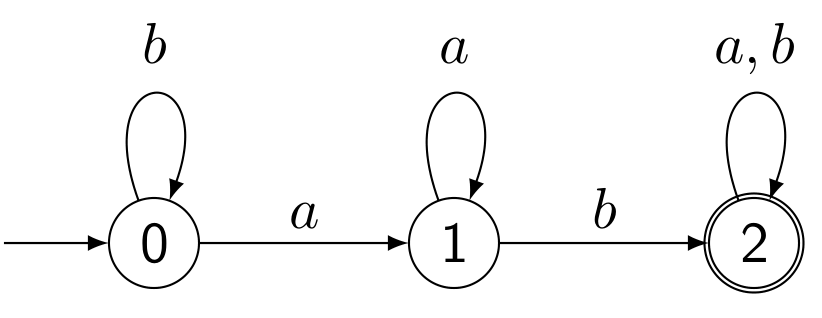
\includegraphics[width=.9\linewidth]{./img/2-kapitel/automat_bsp.png}
\caption{Beispiel Automat}
\end{figure}

\begin{itemize}
\item Beispiel:
\begin{itemize}
\item Eingabewort \(baba \rightarrow\) Zustandsfolge 0,0,1,2,2
\end{itemize}
\item ``Bei dieser Grammatik muss mindestens nach einem a ein b kommen''
\item Die Sprache des DFA ist die Menge aller Wörter über \(\{a,b\}\), die ab enthalten
\end{itemize}

Erkannte Sprache: Menge der Wörter, die vom Startzustand in einen Endzustand führen.
Recognizer, die nur einmal das Wort durchläuft und in linearer Zeit es akzeptiert oder ablehnt.

\subsubsection{Definition}
\label{sec:org374113c}
Ein deterministischer endlicher Automat \(M = (Q,\Sigma, \delta, q_0, F)\) besteht aus
\begin{itemize}
\item endliche Menge von Zuständen Q
\item endlichem Eingabealphabet \(\Sigma\)
\item einer totalen Übergangsfunktion \(\delta: Q \times \Sigma \rightarrow Q\)
\item eienm Startzustand \(q_0 \in Q\)
\item einer Menge \(F \subset Q\) von Endzuständen
\end{itemize}

\begin{enumerate}
\item Akzeptierte Sprachen (Definition 3.2)
\label{sec:orgd8812ff}
Von M akzeptierte Sprache \(L(M) := \{w \in \Sigma^* | \hat{\delta}(q_0, w) \in F\}\) wobei \\
\(\hat{\delta}: Q \times \Sigma^* \rightarrow Q\) induktiv definiert ist: \\
\(\hat{\delta}(q,\epsilon) = q\) \\
\(\hat{\delta}(q,aw) = \hat{\delta}(\delta(q,a),w)\), für \(a \in \Sigma, w \in \Sigma^*\) \\
(\(\hat{\delta}(q, w)\) bezeichnet den Zustand, den man aus \(q\) mit \(w\) erreicht.)\\
Eine Sprache ist regulär \textbf{gdw} sie von einem DFA akzeptiert wird.

\item Beispiel Automat der Sprache akzeptiert
\label{sec:org9d6c74d}
Induktiv beweisen pro Zustand.
\end{enumerate}


\subsection{Von rechtslinearen Grammatiken zu DFA}
\label{sec:orgaf489c8}
\begin{itemize}
\item Für jede rechtslineare Grammatik \(G\) gibt es einen DFA \(M\) mit \(L(M) = L(G)\)
\item Für jeden DFA \(M\) gibt es eine rechtslineare Grammatik \(G\) mit \(L(G) = L(M)\)
\end{itemize}

\subsubsection{Nichtdeterministischer endlicher Automat}
\label{sec:orgd547d76}
Ein deterministischer endlicher Automat \(M = (Q,\Sigma, \delta, q_0, F)\) besteht aus
\begin{itemize}
\item \(Q, \Sigma, q_0, F\) sind wie DFA
\item \(\delta: Q \times \Sigma \rightarrow P(Q)\) \\
\(P(Q)\) = Menge aller Teilmengen von \(Q = 2^Q\) \\
Alternative: Relation \(\delta \subseteq Q \times \Sigma \times Q\)
\end{itemize}


\(\bar{\delta}(S,a) := \bigcup_{q \in S} \delta(q,a)\)


Es folgt: \(\hat{\bar{\delta}}: P(Q) \times \Sigma^* \rightarrow P(Q)\)

\begin{enumerate}
\item Intuition:
\label{sec:org16fde5f}
\(\hat{\bar{\delta}}(S,w)\) ist Menge aller Zustände, die sich von einem Zustand in S aus \(w\) erreichen lassen.

\item Von nichtdeterminitsichen Automaten N akzeptierte Sprache
\label{sec:orge39cfe9}
\(L(N) := \{w \in \Sigma^* | \hat{\bar{\delta}}(\{q_0\},w) \cap F \neq \emptyset\}\)
\end{enumerate}

\subsubsection{Satz 3.9}
\label{sec:org348115c}
Für jede rechtslineare Grammatik G gibt es einen NFA M mit \(L(G) = L(M)\)
\subsubsection{Satz 3.13}
\label{sec:org9b51a29}
Für jeden DFA M gibt es eine rechtslineare Grammatik G mit \(L(M) = L(G)\)

\subsection{3.3 NFAs mit \(\epsilon\) -Übergängen}
\label{sec:org459af2b}
Grammatiken von Programmiersprachen enthalten viele Produktionen der Gestalt \(A \rightarrow B\).

Ein NFA mit \textbf{\(\epsilon\)}-Übergängen (auch \(\epsilon\) -NFA) ist ein NFA mit einem speziellen Symbol \(\epsilon \not \in \Sigma\) und mit
\(\delta : Q \times (\Sigma \cup {\epsilon}) \rightarrow P(Q)\) .
Ein \(\epsilon\) übergang darf ausgef¨uhrt werden, ohne dass ein

\subsubsection{Lemma 3.16}
\label{sec:orgd6da0e5}
Für jeden \(\epsilon\) -NFA \(N\) gibt es einen NFA \(N'\) mit \(L(N) = L(N')\).

\subsection{3.4 Regex}
\label{sec:org3875437}
\begin{itemize}
\item \(\emptyset\) ist ein regex
\item \(\epsilon\) ist ein regex
\item Für jedes \(a \in \Sigma\) ist a ein regulärer Audruck
\item Wenn \(\alpha\) und \(\beta\) regex dann auch
\begin{enumerate}
\item \(\alpha \beta\)
\item \(\alpha | \beta\)
\item \(\alpha^*\)
\end{enumerate}
\item Sonst NIX!
\end{itemize}
\subsubsection{Definition 3.20}
\label{sec:org2460620}
Zu einem regulären Ausdruck \(\gamma\) ist die zugehörige Sprache \(L(\gamma)\) rekursiv definiert:
\begin{itemize}
\item \(L(\emptyset) =\emptyset\)
\item \(L(\epsilon) = \{\epsilon\}\)
\item \(L(a) = {a}\)
\item \(L(\alpha \beta) = L(\alpha)L(\beta))\)
\item \(L(\alpha | \beta) = L(\alpha) \cup L(\beta)\)
\item \(L(\alpha^*) = L(\alpha)^*\)
\end{itemize}

\subsubsection{Satz 3.23 (Kleene 1956)}
\label{sec:org36e794e}
Eine Sprache \(L \subseteq \Sigma^*\) ist genau dann durch einen regulären Ausdruck darstellbar, wenn sie regulär ist.\\
\smallindent
\(R^{k+1}_{ij} = R^k_{ij} \cup R^k_{i(k+1)}(R^k_{(k+1)(k+1)})^*R^k_{(k+1)j}\) \emph{in regex \(\cup = |\)}\\
\(R^{k+1}_{ij}\) = alle Wörter die in \(R^k_{ij}\) sind plus alle Wörter die mindestens einmal \(q_{k+1}\) besuchen
Somit gilt \(L(M) = L(\alpha^n_{1i_1} | ... | \alpha^n_{1i_r})\), wobei \(F=\{i_1, ..., i_r\}\)


\subsubsection{Wie teuer sind unsere Konversionen?}
\label{sec:org1b19c88}
\begin{center}
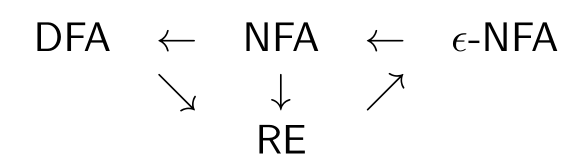
\includegraphics[width=.9\linewidth]{./img/2-kapitel/konversionen.png}
\end{center}
\begin{itemize}
\item RE \(\rightarrow \epsilon\) -NFA: RE der Länge n, \(O(n)\) Zustände
\item \(\epsilon\) -NFA \(\rightarrow\) NFA: Q
\item NFA \(\rightarrow\) DFA: \(O(2^n)\)
\item FA \(\rightarrow\) RE: \(O(n4^n)\)
\end{itemize}

\subsection{Abschlusseigenschaften regulärer Sprachen}
\label{sec:orgcec4bc8}
\subsubsection{Satz 3.24}
\label{sec:org0f556cc}
Seien \(R,R_1, R_2 \subseteq \Sigma^*\) reguläre Sprachen. Dann sind auch
\begin{itemize}
\item \(R_1R_2\)
\item \(R_1 \cup R_2\)
\item \(R^*\)
\item \(\bar{R} (:= \Sigma^* \backslash R)\)
\item \(R_1 \cup R_2\)
\item \(R_1 \backslash R_2\) \\
\end{itemize}
reguläre Sprachen

\begin{enumerate}
\item Produkt-Konstruktion
\label{sec:org8c147aa}
Für den Schnitt ist die De-Morgan regel zu teuer also kann man auch eine Produkt Konstruktion ohne Umweg über De-Morgen benutzen.

Das funktioniert über Parallelismus also beide DFAs laufen synchron parallel (kreuzprodukt der Zustandsräume).
\end{enumerate}

\subsubsection{Satz 3.24 Abschlusseigenschaften regulärer Sprachen}
\label{sec:org1dfb1e3}
Seien \(R. R_1,R_2 \subseteq \Sigma^*\) reguläre Sprachen. Dann sind auch
\(R_1R_2, R_1 \cup R_2, R^k, \bar{R} (:= \Sigma^* \backslash R), R_1 \cap R_2, R_1 \backslash R_2\) auch reguläre Sprachen

\subsubsection{Satz 3.25}
\label{sec:orgc66a018}
Sind \(M_1 = (Q_1, \Sigma,\delta_1,s_1,F_1)\) und \(M_2 = (Q_2,\Sigma,\delta_2,s_s, F_2)\) DFAs, dann ist der \textbf{Produkt-Automat}\\
\indent\indent\indent\indent \(M := (Q_1 \times Q_2, \Sigma, \delta, (s_1,s_2), F_1 \times F_2)\) \\
\indent\indent\indent\indent \(\delta((q_1,q_2), a) := (\delta_1(q_1, a), \delta_2(q_2, a))\)

\subsection{Rechnen mit Regulären Ausdrücken}
\label{sec:org3073155}
\subsubsection{Definition 3.26}
\label{sec:orgbf328fd}
Zwei reguläre Ausdrücke sind \textbf{äquivalent gdw} sie die gleiche Sprache darstellen:
\(\alpha \equiv \beta: \Leftrightarrow L(\alpha) = L(\beta)\)

(by the way \(\equiv\) steht für Bedeutungsäquivalenz und \(=\) für syntaktische gleichheit)

\subsubsection{Lemma 3.27}
\label{sec:org1d79807}
\begin{itemize}
\item \(\emptyset | \alpha \equiv \alpha | \emptyset \equiv \alpha\)
\item \(\emptyset \alpha \equiv \alpha\emptyset \equiv \emptyset\)
\item \(\epsilon\alpha \equiv \alpha\epsilon \equiv \alpha\)
\item \(\emptyset^* \equiv \epsilon\)
\item \(\epsilon^* \equiv \epsilon\)
\end{itemize}

\subsubsection{Lemma 2.8}
\label{sec:org6db4d95}
\begin{itemize}
\item Assozitiviät
\item Kommutativität
\item Distributivität
\begin{itemize}
\item \(\alpha(\beta | \gamma) \equiv \alpha\beta | \alhpa\gamma\)
\item \((\alpha | \beta)\gamma \equiv \alpha\gamma | \beta\gamma\)
\end{itemize}
\item Idempotenz: \(\alpha | \alpha \equiv \alpha\)
\end{itemize}

\subsection{Pumping Lemma}
\label{sec:org8abf3cd}
Wie zeigt man, dass eine Sprache nicht regulär ist?
\subsubsection{Satz 3.32 (Pumping Lemma für Reguläre Sprachen)}
\label{sec:org1e3ee56}
Sei \(R \subseteq \Sigma^*\) regulär. Dann gibt es ein \(n > 0\), so dass sich jedes \(z \in R\) mit \(|z| \geq n\) so in \(z = uvw\) zerlegen lässt, dass
\begin{itemize}
\item \(v \neq \epsilon\),
\item \(|uv| \leq n\)
\item \(\forall i \geq 0. uv^iw \in R\). \\
\end{itemize}

Es gibt nicht-reguläre Sprachen, für die das Pumping-Lemma gilt!
\(\Rightarrow\) Pumping-Lemma hinreichend aber nicht notwendig um Nicht-Regularität zu zeigen.

regulär  \(\subset\) Pumping-Lemma gilt \(\subset\) alle Sprachen

\subsection{Entscheidungsverfahren}
\label{sec:org21bcb90}

\textbf{Eingabe:} Ein oder mehrere Objekte, die Reguläre Sprachen beschreiben (DFA, NFA, RE Typ3 Gram, \ldots{})
\textbf{Frage:} Haben die Sprachen die Eigenschaft X?
Ein (Entscheidungs-)Problem ist entscheidbar, wenn es einen Algorithmus gibt, der bei jeder Eingabe in endlicher Zeit die richtige Antwort auf die Frage feststellt.

Welche Entscheidungsprobleme sind für rechtslineare Grammatiken entscheidbar und wie hängt die Laufzeit mit der Beschreibung zusammen.

\subsubsection{Definition 3.37}
\label{sec:org487e9d0}
Sei D ein DFA, NFA, RE, rechtslineare Grammatik \ldots{}
\begin{itemize}
\item \textbf{Wortproblem}: Gegeben \(w\) und D: gilt \(w \in L(D)\)
\item \textbf{Leerheitsproblem}: Gegeben D: gilt \(\emptyset = L(D)\)
\item \textbf{Endlichkeitsproblem}: Gegeben D: isz \(L(D)\) endlich
\item \textbf{Äquivalenzproblem}: Gegeben \(D_1, D_2\), gilt \(L(D_1) = L(D_2)\)
\end{itemize}

\subsection{Automaten und Gleichungssysteme}
\label{sec:org8e5b1b0}
Wir werden jetzt aus einem Automat ein Gleichungssystem machen um daraus einen RE zu machen.

\subsubsection{Ardens Lemma (Satz 3.47)}
\label{sec:orgcefd485}
Sind A, B und X Sprachen mit \(\epsilon \not \in A\), so gilt
\(X = AX \cup B \Rightarrow X = A^*B\)
\subsubsection{Korollar 3.48}
\label{sec:orgb6b53a0}
Sind \(\alpha, \beta\) und X reguläre Ausdrücke mit \(\epsilon \not \in L(\alpha)\), so gilt
\(X \equiv  \alpha X|\beta \Rightarrow X \equiv \alpha^*\beta\)
\subsubsection{Algorithmus um RE aus Automat zu machen}
\label{sec:org78fd02a}

\begin{enumerate}
\item Wandle FA mit n Zuständen in ein System von n Gleichungen
\item Löse das System durch schrittweise Elimination von Variablen mit Hilfe von Ardens Lemma für REs (Korollar 3.48).
\item Ist k der Startzustand, so beschreibt X\textsubscript{k} die vom Automaten akzeptierte Sprache.
\end{enumerate}

\subsection{Minimierung endlicher Automaten}
\label{sec:org94b7561}
\textbf{TODO MIA}

\subsection{Äquivalenztest von DFAs}
\label{sec:org2969956}
Zwei Automaten sind genau äquivalent wenn:
\begin{enumerate}
\item Gegeben DFAs \(M1\) und \(M2\), bilde disjunkte Vereiningung. \\
(”Male M1 und M2 nebeneinander.“)
\item Berechne Menge der äquivalenten Zustände.
\item L(M1) = L(M2) gdw die beiden Startzustände äquivalent sind
\end{enumerate}

\subsection{Äquivalenz von Zuständen}
\label{sec:orge0923fb}
Zwei Zustände sind äquivalent wenn sie selbe Sprache akzeptieren.


\subsection{Minimalität des Quotientenautomaten}
\label{sec:orgb350c99}

Die Residualsprache von L bzgl \(w \in \Sigma^*\) ist die Menge:

\(L^w := \{z \in \Sigma^* | wz \in L\}\)

\(L' \subseteq \Sigma^*\) ist Residualsprache von L wenn es \(w\) gibt mit \(L' = L^w\)

\subsubsection{Definition 3.55 (Äquivalenz von Wörtern bzgl. L)}
\label{sec:org5fbe5ae}
(Intuition: Zwei Wörter sind äquivalent wenn sie die gleiche Residualsprache haben.)

\textbf{zwei Wörter sind äquivalent gdw sie zu den gleichen Zuständen führen}

\subsubsection{Satz 3.56}
\label{sec:orgfa3343f}
Sei M ein DFA ohne unerreichbare Zustände. Der Quotientenautomat \(M / \equiv\) ist ein minimaler DFA für \(L(M)\).

\subsection{Definition 3.57 (Kanonischer Minimalautomat)}
\label{sec:orgce0755d}
\(M_L := (R_L, \Sigma, \delta_L, L, F_L)\)
mit \(\delta_L(R, a) := R^a\) und \(F_L := {R \in RL | \varepsilon \in R}\).
\(\delta_L\) ist wohldefiniert und \(\hat{\delta}}_L(R, w) = R^w\). Jeder Zustand \(R\) erkennt
die Sprache \(R\) und somit \(L(M_L) = L\).
\subsubsection{Satz 3.58}
\label{sec:org761036d}
Jeder minimaler DFA für eine reguläre Sprache L unterscheidet sich vom kanonischen Minimalautomaten M\textsubscript{L} nur durch eine
\subsection{Satz 3.59}
\label{sec:org4429ef2}
Eine Sprache \(L \subseteq \Sigma^*\) ist genau dann regulär, wenn sie endlich viele Residualsprachen hat.

\section{Kontextfreie Sprachen}
\label{sec:orga61e0fd}
\subsubsection{Syntaxbaum:}
\label{sec:org7f886ef}
Die Blätter des Baums, von links nach rechts gelesen,
\subsection{Definition 4.2}
\label{sec:orgfea75e4}
Eine kontextfreie Grammatik \(G = (V, \Sigma, P, S)\) ist ein 4-Tupel: \\
\(V\) ist eine endlichen Menge, die Nichtterminalzeichen (oder Variablen), \\
\(\Sigma\) ist ein Alphabet, die Terminalzeichen, disjunkt von V ,
\(P \subseteq V \times (V \cup Σ´\Sigma)*\) eine endlichen Menge, die Produktionen, und \\
\(S \in V\) ist das Startsymbol.
\subsection{Definition 4.4}
\label{sec:org3e2770f}
Eine kontextfreie Grammatik G = (V, Σ, P, S) induziert eine
Ableitungsrelation →G auf W¨ortern ¨uber V ∪ Σ:
α →G β
gdw es eine Regel A → γ in P gibt, und W¨orter α1, α2, so dass
α = α1Aα2
und
β = α1γα2
Beispiel:
a + T + a
→G

\subsection{Definition 4.5 (Reflexiv transitive Hülle)}
\label{sec:org9cb768c}
TODO

\subsection{Definition 4.6 (Kontextfreie Sprache)}
\label{sec:orgff37a46}
TODO

\subsection{Lemma 4.9 (Dekompositionslemma)}
\label{sec:org1586f35}
\(\alpha_1 \alpha_2 \rightarrow^n_G \beta\) \\
\(\Leftrightarrow\) \\
\(\exists \beta_1, \beta_2, n_1, n_2. \beta = \beta_1\beta_2 \land n = n_1 + n_2 \land \alpha_i \rightarrow^{n_i}_G \beta_i (i = 1, 2)\)

\subsection{Definition 4.12 (Balancierte Klammerausdrücke)}
\label{sec:orgb30a1dc}
\subsubsection{Präfix}
\label{sec:org9df42d7}
\(u \preceq w \iff \exists v : uv = w\)
\subsubsection{Anzahl an Vorkommnissen}
\label{sec:org903f078}
\(\#_a(w) :=\) Anzahl an \(a\)'s in \(w\)
Seien \(A(w) := \#_[(w) \quad B(w) := \#_](w)\)
\(w\in \{\ [\ ,\ ]\ \}^*\) sei \textbf{balanciert} gdw
\begin{enumerate}
\item \(A(w) = B(w)\)
\item \(\forall u \preceq w : A(u) \geq B(u)\)
\end{enumerate}
\subsubsection{4,13}
\label{sec:org581e420}
Grammatik \(S \rightarrow \epsilon\ |\ [S]\ |\ SS\) erzeugt genau die Menge der balancierten Wörter

\subsection{4.15 Syntaxbaum}
\label{sec:org0839136}
Ein Syntaxbaum für \(G = \{V, \Sigma, P, S)\}\) so dass gilt:
\begin{itemize}
\item jedes Blatt mit einem Zeichen aus \(\Sigma \cup \{\epsilon\}\) beschriftet ist
\item jeder innere Knoten mit einem \(A\in V\) beschriftet ist, falls Nachfolger: als \(X_1, ..., X_n \in V\cup \Sigma \cup \{\epsilon\}\) beschriftet. Dann ist \(A \rightarrow X_1, ..., X_n\) eine Produktion in \(P\)
\item ein Blatt \(\epsilon\) der einzige Nachfolger seines Vorgänger ist
\end{itemize}

\subsection{4.17 Äquivalente Bedingungen}
\label{sec:orgff60ba7}
Für ein CFG \& \(w \in \Sigma^*\)
\begin{itemize}
\item \(A\rightarrow_G^* w\)
\item \(w\in L_G(A)\) (gemäß der induktiven Definition)
\item Es gibt ein Syntaxbaum mit Wurzel A dessen \textbf{Rand} das Wort \emph{w} ist
\end{itemize}

\subsection{4.18}
\label{sec:orge0d79da}
Ein CFG heißt mehrdeutig \(\iff\) es 2 \textbf{verschiedene} Syntaxbäume gibt die mit gleichem Rand \\
Ein CFL L heißt inhärent mehrdeutig \(\iff\) jede CFG G mit \(L(G) = L\) mehrdeutig ist

\section{Chomsky-Normalform}
\label{sec:org8456298}
\subsubsection{4.21}
\label{sec:orge92e2f8}
Ein CFG G ist in Chomsky-Normalform \(\iff\) alle Produktionen eine der Formen:
\(\qquad A \rightarrow a\quad\) oder \(\quad A\rightarrow BC\quad\) haben
\subsubsection{4.22}
\label{sec:orgf1fa605}
Jede CFG G hat eine CFG \(G'\) in Chomsky-Normalform mit \(L(G') = L(G) \backslash \{\epsilon\}\)
Wenn man \(\epsilon \in L(G')\) haben will: Füge am Ende \(S' \rightarrow S, S\rightarrow \epsilon\) hinzu und setzte \(S'\) als Startsymbol

\subsubsection{Beispiel mit Farben weil Noah immernoch nicht versteht}
\label{sec:org5c35481}
\begin{center}
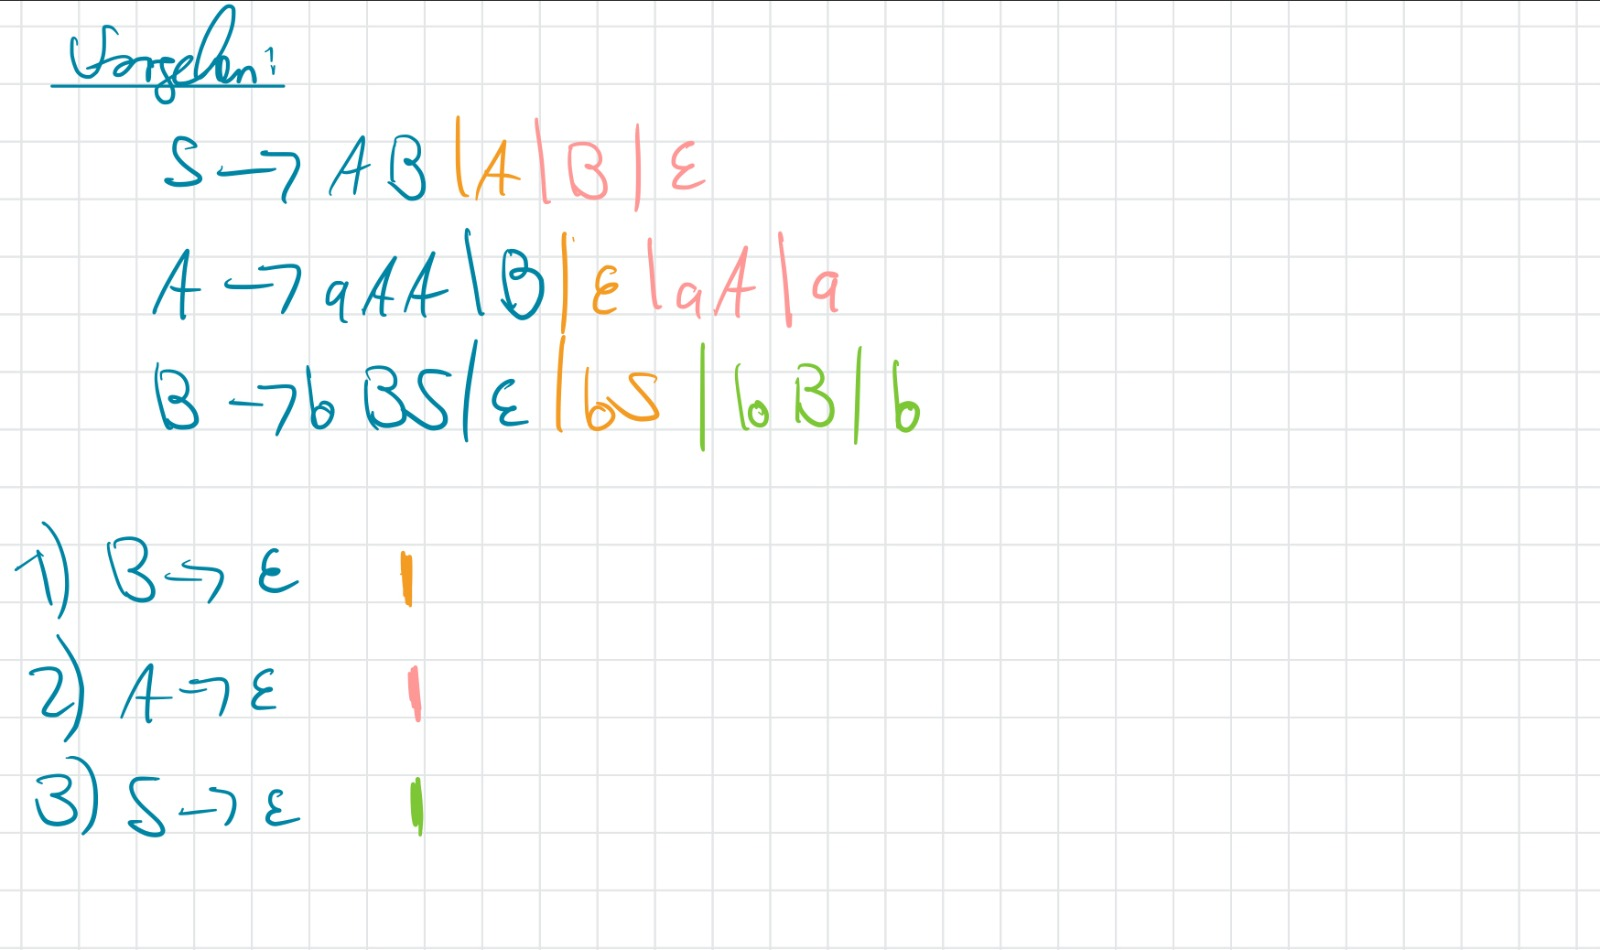
\includegraphics[width=.9\linewidth]{./img/3-kapitel/chomskybsp.png}
\end{center}

\(A\rightarrow B\) ist eine \textbf{Kettenproduktion}
\subsection{4.25}
\label{sec:orga98bd9d}
Aus jeder CFG G kann man ein CFG G' konstruieren was keine Kettenproduktionen enthält sodass gilt \$L(G) = L(G')

\subsubsection{Beispiel Kettenproduktionen:}
\label{sec:org1940bbd}
\begin{center}
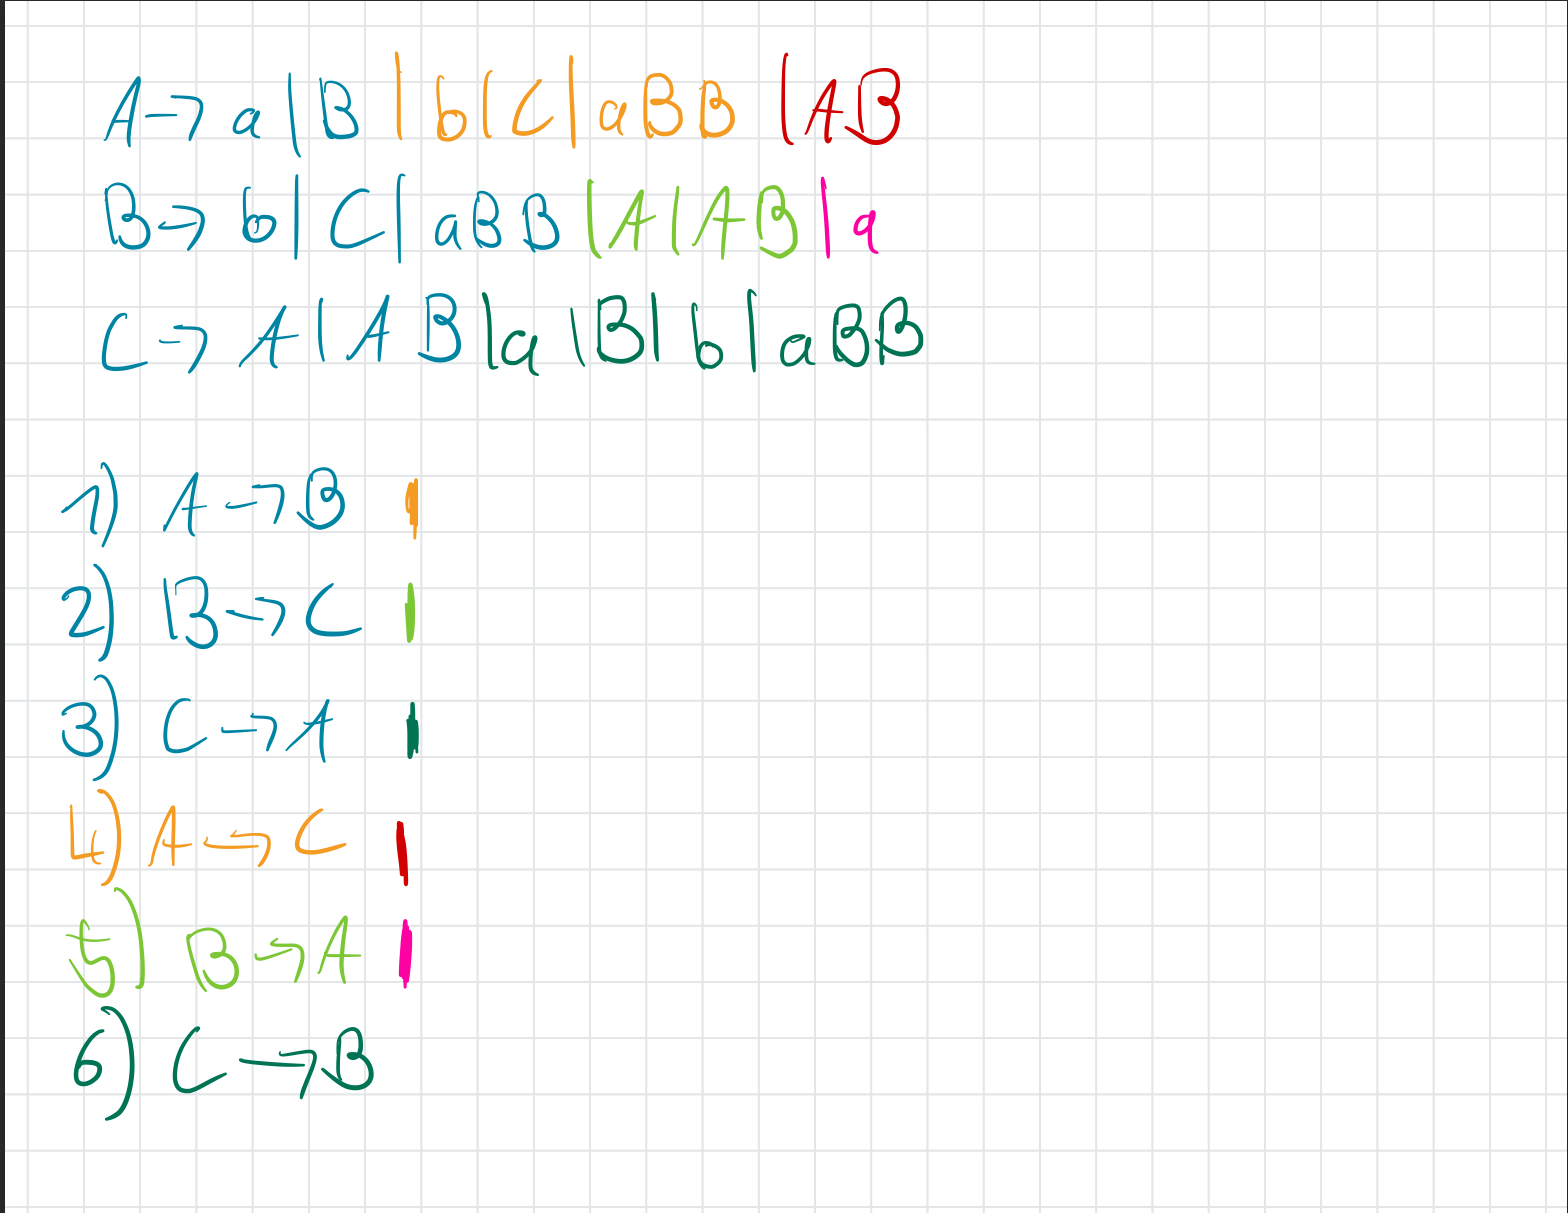
\includegraphics[width=.9\linewidth]{./img/3-kapitel/chomskybsp2.png}
\end{center}

\subsection{Konstruktion einer Chomsky-Normalform}
\label{sec:org90f6a8b}
Eingabe: eine kontextfreie Grammatik \(G = (V, \Sigma, P, S)\)
\begin{enumerate}
\item Für jedes \(a\in \Sigma\) das in einer Produktion mit Länge \(\ge\) 2 vorkommt:
\begin{itemize}
\item Füge ein neues Nichtterminal \(X_a\) zu \(V\) \& ersetzt alle diese a's dadurch
\item Füge \(X_a \rightarrow a\) zu \(P\) hinzu
\end{itemize}
\item Ersetze Produktion in der Form: \\
\begin{center}
\(A\rightarrow B_1B_2...B_k\quad (k\ge 3)\)
\end{center}
durch \\
\begin{center}
\(A\rightarrow B_1C_2,\ C_2\rightarrow B_2C_3,\ ...,\ C_{k-1}\rightarrow B_{k-1}B_k\) \\
\end{center}
wobei \(C_2,\ ...,\ C_{k-1}\) neue Nichtterminale sind
\item Elimniere alle \(\epsilon\) -Produktionen
\item Eliminiere alle Kettenproduktionen
\end{enumerate}

\subsection{4.27 Greibach-Normalform}
\label{sec:orgb9d875b}
Ein CFG ist in Greibach-Normalform falls alle Produktionen in der From sind: \\
\(A\rightarrow aA_1...A_n\)

\subsubsection{Satz 4.28}
\label{sec:org9263f02}
Zu jeder CFG G gibt es eine CFG \(G′\) in Greibach-Normalform mit \\
\(L(G') = L(G) \backslash \{\epsilon\}\).

\subsection{Pumping Lemma für kontextfreie Sprachen}
\label{sec:org9232baf}
Für jede kontextfreie Sprache L gibt es ein \(n \ge 1\), so dass sich jedes Wort \(z\in L\) mit \(|z| \ge n\) sich zerlegen lässt in: \\
\(z = uvwxy\) \\
mit
\begin{itemize}
\item \(vx \ne \epsilon\)
\item \(|vwx| \le n\)
\item \(\forall i \in \mathbb{N} : uv^iwx^iy\in L\)
\end{itemize}

\subsection{Abschlusseigenschaften kontextfreie Sprachen}
\label{sec:org25295f7}
Die Klasse der kontextfreien Sprachen ist also unter Vereinigung, Konkatenation, Stern und Spiegelung abgeschlossen. (Genau wie reguläre Sprachen)
\subsection{Algorithmen für kontextfreie Grammatiken}
\label{sec:orgf13abbe}
\(G\) sei eine CFG
Ein Symbol \(X \in V \cup \Sigma\) ist
\begin{itemize}
\item \textbf{nützlich} gdw es eine Ableitung \(S \rightarrow^*_G w \in \Sigma^*\) gibt in der \(X\) vorkommt.
\item \textbf{erzeugend} gdw es eine Ableitung X \(\rightarrow\)\textsuperscript{*}\textsubscript{G} w \(\in\) \(\Sigma\)\textsuperscript{*}\$ gibt.
\item \textbf{erreichbar} gdw es eine Ableitung \(S \rightarrow^*_G \alpha X \beta\)
\end{itemize}
\subsubsection{Satz 4.36}
\label{sec:org2f5c6af}
Eliminiert man aus einer Grammatik \(G\)
\begin{enumerate}
\item alle nicht erzeugenden Symbole, mit Resultat \(G_1\), und
\item aus \(G_1\) alle unerreichbaren Symbole, mit Resultat \(G_2\),
\end{enumerate}

dann enthält \(G_2\) nur noch nützliche Symbole und \(L(G_2) = L(G)\).

\subsubsection{Satz 4.37}
\label{sec:orgb42b9b2}
Die Menge der erzeugenden Symbole einer CFG sind berechenbar
\subsubsection{Satz 4.38}
\label{sec:org77dd461}
Für eine CFG ist entscheidbar, ob \(L(G) = \emptyset\)
\subsubsection{Satz 4.40}
\label{sec:orga1aeeac}
Die Menge der erreichbaren Symbole einer CFG ist berechenbar.

\subsection{Der Cocke-Younger-Kasami-Algorithmus}
\label{sec:org1aec889}
Der CYK-Algorithmus entscheidet das Wortproblem für kontextfreie Grammatiken in Chomsky-Normalform.
Eingabe: Grammatik in Chomsky-Normalform,
\(w = a_1 ... a_n \in \Sigma^*\)
\subsubsection{Definition 4.42}
\label{sec:org565b92c}
\(V_{ij} := \{A \in V | A \rightarrow^*_G a_i...a_j\}\) für \(i \geq j\) \\
Damit gilt: \\
\(w \in L(G) \iff S \in V_{1n}\)
\subsubsection{Satz 4.44}
\label{sec:org445a455}
Der CYK-Algorithmus entscheidet das Wortproblem \(w \in L(G)\) für eine fixe CFG G in Chomsky-Normalform in Zeit \(O(|w|^3)\).

\subsubsection{Vorschau}
\label{sec:org48e3088}
Für CFGs sind folgende Probleme nicht entscheidbar:
\begin{itemize}
\item Äquivalenz: \(L(G_1) = L(G_2)\)?
\item Schnittproblem: \(L(G_1) \cap L(G_2) = \emptyset\)?
\item Regularität: \(L(G)\) regulär?
\item Mehrdeutigkeit: Ist \(G\) mehrdeutig?
\end{itemize}

\subsection{Kellerautomaten}
\label{sec:org6344033}
Ein (nichtdeterministischer) Kellerautomat \\
\(M = (Q, \Sigma, \Gamma, q_0, Z_0, \delta, F)\) besteht aus \\
\begin{itemize}
\item einer endlichen Menge von Zuständen \(Q\),
\item einem endlichen Eingabealphabet \(\Sigma\),
\item einem endlichen Kelleralphabet \(\Gamma\),
\item einem Anfangszustand \(q_0\),
\item einem untersten Kellerzeichen \(Z_0\),
\end{itemize}
einer Übergangsfunktion \(\delta: Q \times (\Sigma \cup \{\epsilon\}) \times \Gamma \rightarrow \mathcal{P}_e(Q \times \Gamma^*)\) , \\
(Hierbei bedeutet \(\mathcal{P}_e\) die Menge aller endlichen Teilmengen)
\begin{itemize}
\item einer Menge \(F \subseteq Q\) von Endzuständen.
\end{itemize}
\subsubsection{Spezialfälle}
\label{sec:org6ac225d}
\begin{itemize}
\item POP-Operation: \(\alpha = \epsilon\)
Das oberste kellerzeichen \(Z\) wird entfernt.
\item PUSH-Operation: \(\alpha = Z'Z\)
Z′ wird als neues oberstes Kellerzeichen gePUSHt
\item \(\epsilon\) -Übergang: \(a = \epsilon\)
Ohne Lesen eines Eingabezeichens.
\end{itemize}
\subsubsection{Definition 4.48}
\label{sec:org5f1bfdf}
\begin{itemize}
\item Ein PDA \(M\) \textbf{akzeptiert} \(w \in \Sigma^*\) mit \textbf{Endzustand} gdw \\
\((q_0, w, Z_0) \rightarrow^*_M (f, \epsilon, \gamma)\) für ein \(f \in F, \gamma \in \Gamma^*\). \\

\(L_F(M) := \{w | \exists f \in F, \gamma \in \Gamma^*. (q_0, w, Z_0) \rightarrow^*_M (f,\epsilon,\gamma)\}\)

\item Ein PDA \(M\) \textbf{akzeptiert} \(w \in \Sigma^*\) \textbf{mit leerem Keller} gdw
\((q_0, w, Z_0) \rightarrow^*_M (q, \epsilon, \epsilon)\) für ein \(q \in Q\). \\

\(L_\epsilon(M) := \{w | \exists q \in Q. (q_0, w, Z_0) \rightarrow^*_M (q,\epsilon,\epsilon)\}\)
\end{itemize}

\subsubsection{Satz 4.50 (Endzustand → leerer Keller)}
\label{sec:orgf7ae9a4}
Zu jedem PDA \(M = (Q, \Sigma, \Gamma, q_0, Z_0, \delta)\) kann man in linearer \\
Zeit einen PDA \(M' = (Q', \Sigma, \Gamma', q'_0, Z'_0, \delta′)\) konstruieren mit \\
\(L_F(M) = L_\epsilon(M')\)

\subsubsection{Satz 4.51 (Leerer Keller → Endzustand)}
\label{sec:orgb5196ea}
Zu jedem PDA \(M\) kann man in linearer Zeit einen PDA \(M'\) konstruieren mit \\
\(L_\epsilon(M) = L_F(M')\)

\subsubsection{Lemma 4.52 (Erweiterungslemma)}
\label{sec:org44a731f}
\((q, u, \alpha) \rightarrow^n_M (q', u', \alpha') \implies (q, uv, \alpha \beta) \rightarrow^n_M (q', u'v, \alpha'\beta)\) \\
Intuitiv: Man kann bei einem kellerautomaten unten beliebig viele elemente hinzufügen weil sie demnach eh nie gelesen werden.

\subsubsection{Zerlegungssatz}
\label{sec:org1603ade}
Wenn \((q, w, Z_{1...k}) \rightarrow^n_M (q', \epsilon, \epsilon)\)
dann gibt es \(u_i, p_i, n_i\), so dass
\((p_{i−1}, u_i, Z_i) \rightarrow^{n_i}_M (p_i, \epsilon, \epsilon) (i = 1, . . . , k)\)
und \(w = u_1 . . . u_k, p_0 = q, p_k = q', \sum n_i = n\).
\begin{center}
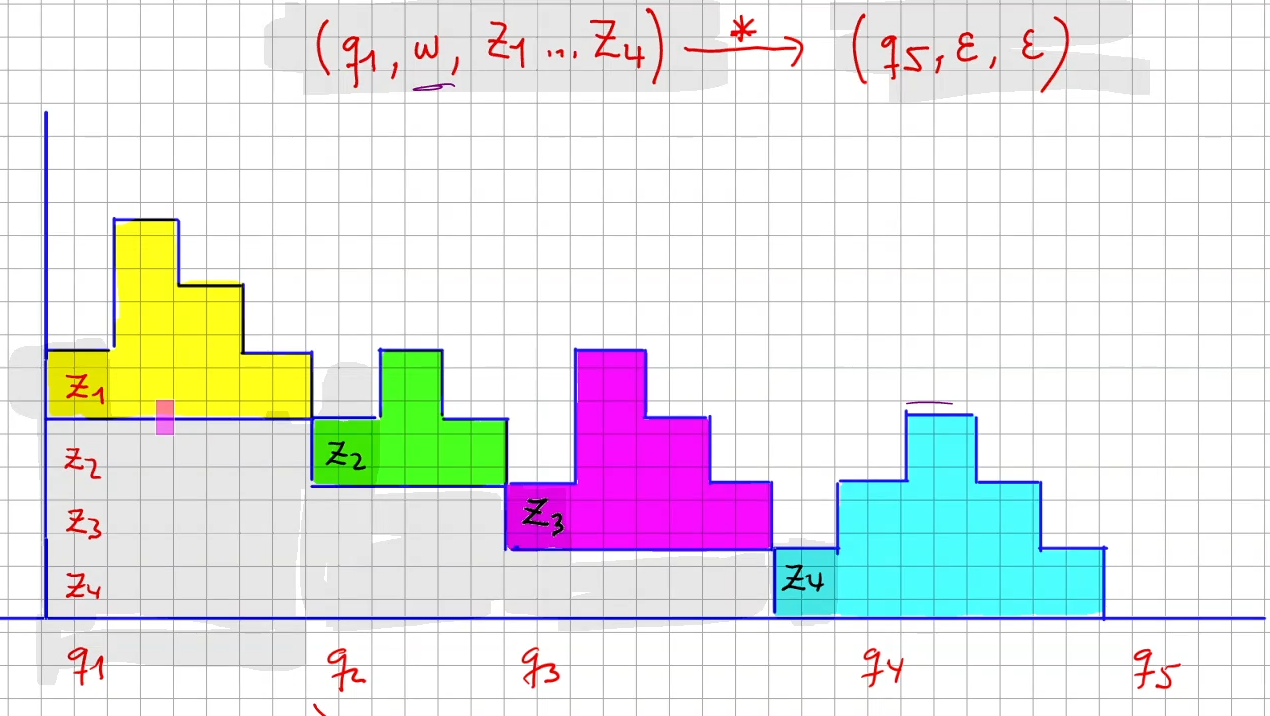
\includegraphics[width=.9\linewidth]{./img/3-kapitel/zerlegungssatz.png}
\end{center}

\subsubsection{Satz 4.54 (CFG → PDA)}
\label{sec:orge755796}
Zu jeder CFG \(G\) kann man einen PDA \(M\) konstruieren, der mit leerem Stack akzeptiert, so dass \(L_\epsilon(M) = L(G)\).
\subsubsection{Satz 4.57 (PDA → CFG)}
\label{sec:org4f3356b}
Zu jedem PDA \(M = (Q, \Sigma, \Gamma, q_0, Z_0, \delta)\), der mit leerem Keller
akzeptiert, kann man eine CFG \(G\) konstruieren mit \(L(G) = L_\epsilon(M)\).
\subsubsection{Satz 4.59}
\label{sec:org6d81a07}
\textbf{Eine Sprache ist kontextfrei gdw sie von einem Kellerautomaten}

\subsection{Deterministische Kellerautomaten}
\label{sec:org97707f3}
\subsubsection{Definition 4.60}
\label{sec:org1551653}
Ein PDA heißt deterministisch (DPDA) gdw für alle \(q \in Q, a \in \Sigma, Z \in \Gamma\) \\
\(|\delta(q, a, Z)| + |\delta(q, \epsilon, Z)| \leq 1\)
\subsubsection{Definition 4.62}
\label{sec:org9dd3d70}
Eine CFL heißt deterministisch (DCFL) gdw sie von einem DPDA
akzeptiert wird.
\subsubsection{Fakt 4.63}
\label{sec:org77bd031}
Jede reguläre Sprache ist eine DCFL.
\subsubsection{Lemma 4.65}
\label{sec:org9f93e3f}
\(\exists\) DPDA \(M. L = L_\epsilon(M)\) \\
\(\iff\) \\
\(\exists\) DPDA \(M. L = L_F(M)\) und \(L\) erfüllt die Präfix Bedingung
\subsubsection{Satz 4.66}
\label{sec:org313e139}
Die Klasse der DCFLs ist unter Komplement abgeschlossen. \\
(CFLs sind nicht unter Komplement abgeschlossen)
\subsubsection{Lemma 4.68}
\label{sec:org9320864}
Die Klasse der DCFLs ist weder unter Schnitt noch unter
Vereinigung abgeschlossen. \\
(CFLs auch nicht)
\subsubsection{Lemma 4.69}
\label{sec:org244118b}
Jede DCFL ist nicht inhärent mehrdeutig, dh sie wird von einer
nicht-mehrdeutigen Grammatik erzeugt.
\subsubsection{Satz 4.70}
\label{sec:org76d8fed}
Das Wortproblem für DCFLs ist in linearer Zeit lösbar.
\end{document}
